\documentclass[10pt, a4paper,spanish]{article}

\usepackage{./mystyle}
\usepackage{./myvars}



%-----------------------------

\begin{document}

	\maketitle % Insert title

	\thispagestyle{fancy} % All pages have headers and footers


%-----------------------------
%	ABSTRACT
%-----------------------------

	\begin{abstract}
		\noindent Abstract
	\end{abstract}

%-----------------------------
%	TEXT
%-----------------------------


  \section{Tómese la siguiente función lógica y obténgase el árbol de decisión correspondiente usando WEKA}

		\begin{equation}
			\label{eq:logic_equation}
			\neg(A \land B) \lor \neg(C \land D) \oplus E
		\end{equation}

		\paragraph{}
		En esta práctica se ha generado la tabla de verdad de la función descrita en la ecuación \eqref{eq:logic_equation}. Por lo tanto, el conjunto de datos que se ha utilizado en este caso sigue la siguiente estructura:
		\begin{enumerate*} [label=\itshape\alph*\upshape)]
			\item los atributos de cada dato se corresponden con una determinada combinación de las variables de entrada de \eqref{eq:logic_equation},
			\item mientras que el valor de la clase será el valor de verdad de dicha combinación.
		\end{enumerate*}

		\paragraph{}
		El conjunto de datos está compuesto por tanto, por 5 atributos de tipo booleano (discretos) al igual que la clase, que también es de tipo booleano. Puesto que la función está formada por 5 argumentos y cada uno de ellos puede tomar 2 valores, nuestro conjunto de datos está formado por $2 ^ 5 = 32$ datos. Todos ellos han sido recogidos en la tabla \ref{eq:truth_table}. Dicha tabla de verdad ha sido generada a partir de la clase \emph{LogicDataSet} codificada en el lenguaje \emph{Python}, a la cual se puede acceder a partir de \url{https://github.com/garciparedes/python-examples/blob/master/data_sets/logic_data_set.py}\cite{github:garciparedes-python-examples}.


		\paragraph{}
		El propósito de esta práctica es analizar el comportamiento de las estrategias de aprendizaje automático básadas en estructuras jerárquicas (árboles). Para ello se ha utilizado la herramienta \emph{Weka}, que permite la realización de diversas tareas relacionadas con el aprendizaje automático de manera simple y de manera gráfica sobre conjuntos de datos. En este caso se ha realizado una comparativa entre los algoritmos de clasificación basada en árboles mediante aprendizaje supervisado.

		\paragraph{}
		Debido a la naturaleza intrínseca de un estructura en forma de árbol, esto permiten la representación de funciones lógicas con un alto grado de acierto. Para comprobar dicha cualidad, se ha realizado un ánalisis de resultados de los algoritmos \emph{ID3} y \emph{J48}, cuyas diferencias son las siguientes:

		\begin{itemize}

			\item \textbf{ID3}: Es el algoritmo básico de generación de árboles de decisión a partir de un conjunto de datos formado tanto por atributos como valores de clase de carácter discreto. Utiliza heurísticas basadas en la Teoría de Información. Debido a sus simplicidad, está muy condicionado al conjunto de datos de entrenamiento.

			\item \textbf{J48}: Es la versión implementada en el lenguaje \emph{Java} del algoritmo \textbf{C4.5}, una versión con numerosas mejoras respecto de \emph{ID3}, tales como:
				\begin{enumerate*}[label=\itshape\alph*\upshape)]
					\item la capacidad de procesar atributos continuos mediante la generación,
					\item manejo de valores desconocidos,
					\item mismos atributos de entrada para distintos valores para la clase de destino y
					\item poda para tratar de evitar el sobreajuste.
				\end{enumerate*}
		\end{itemize}

		\paragraph{}
		Para los casos de prueba, en los dos casos se han utilizado los parámetros por defecto de la herramienta \emph{Weka}. Tras utilizar todo el conjunto de datos tanto para entrenamiento como para test, los árboles generados por el algoritmo \textbf{ID3} y \textbf{J48} se muestran en las figuras \ref{fig:id3-tree} y \ref{fig:j48-tree}. Dichas figuras han sido generadas a partir de la herramienta \emph{treetograph}\cite{github:ismtabo-treetograph}.


		\paragraph{}


		\paragraph{}


		\begin{table}[p]
			\begin{center}
				\csvautotabular{data.csv}
			\end{center}
			\caption{Tabla de verdad de la ecuación \ref{eq:logic_equation}}
			\label{eq:truth_table}
		\end{table}


		\begin{figure}[h]
			\begin{center}
				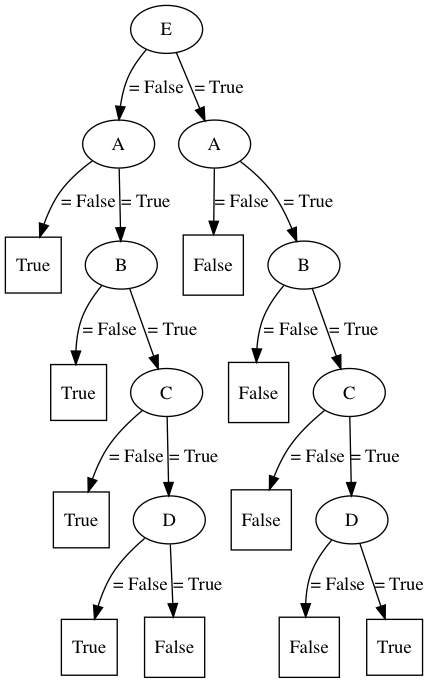
\includegraphics[width=0.5\textwidth]{id3-tree}
			\end{center}
			\caption{Árbol de decisión generado a partir del algoritmo \emph{ID3}}
			\label{fig:id3-tree}
		\end{figure}

		\begin{table}{h}
			\begin{center}
				\begin{tabular}{r c c|c|l}
					& & \multicolumn{2}{ c }{Valor Real} \\ \cline{3-4}
					& & \multicolumn{1}{ |c| }{Positivo} & \multicolumn{1}{ |c| }{Negativo} & \multicolumn{1}{ l }{$p_j$}\\ \cline{2-4}
					\multicolumn{1}{  c  }{\multirow{2}{*}{Valor Predicho} } 	& \multicolumn{1}{ |c| }{Positivo} & $15$ & 1 &  $0.9375$   \\ \cline{2-4}
					\multicolumn{1}{  c  }{}                        					& \multicolumn{1}{ |c| }{Negativo} & $1$  & 15 & $0.9375$ \\ \cline{2-4}
					& \multicolumn{1}{ c }{$\pi_j$} & \multicolumn{1}{ c }{$0.5$} & \multicolumn{1}{ c }{$0.5$} & \multicolumn{1}{ l }{$N = 32$}
				\end{tabular}
			\end{center}
			\caption{Resultados J48}
			\label{}
		\end{table}

		\begin{figure}[h]
			\begin{center}
				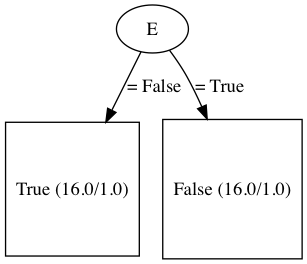
\includegraphics[width=0.5\textwidth]{j48-tree}
			\end{center}
			\caption{Árbol de decisión generado a partir del algoritmo \emph{J48}}
			\label{fig:j48-tree}
		\end{figure}

		\begin{table}{h}
			\begin{center}
				\begin{tabular}{r c c|c|l}
					& & \multicolumn{2}{ c }{Valor Real} \\ \cline{3-4}
					& & \multicolumn{1}{ |c| }{Positivo} & \multicolumn{1}{ |c| }{Negativo} & \multicolumn{1}{ c }{$p_j$}\\ \cline{2-4}
					\multicolumn{1}{  c  }{\multirow{2}{*}{Valor Predicho} } 	& \multicolumn{1}{ |c| }{Positivo} & $16$ & $0$ &  $1$   \\ \cline{2-4}
					\multicolumn{1}{  c  }{}                        					& \multicolumn{1}{ |c| }{Negativo} & $0$  & $16$ & $1$ \\ \cline{2-4}
					& \multicolumn{1}{ c }{$\pi_j$} & \multicolumn{1}{ c }{$0.5$} & \multicolumn{1}{ c }{$0.5$} & \multicolumn{1}{ c }{$N = 32$}
				\end{tabular}
			\end{center}
			\caption{Resultados ID3}
			\label{}
		\end{table}

%-----------------------------
%	Bibliographic references
%-----------------------------
	\nocite{subject:taa}
  \bibliographystyle{acm}
  \bibliography{bib/misc}

\end{document}
